%==============================================================================%
% SERIALIZABILITY & LOCKING                                                    %
%==============================================================================%

\section{Serializability \& Locking}

\begin{multicols}{2}
    In schedule 1 we see that $T_1$ reads $X$ whilst $T_2$ wants to write to
    $X$, so $T_1$ must wait for $T_2$. $T_2$ also wants to write to $Z$ whilst
    $T_3$ wants to read $Z$, so $T_2$ must wait for $T_3$. $T_3$ reads $Y$
    whilst $T_1$ wants to write to $Y$, so $T_3$ must then wait for $T_1$.
    \begin{figure}[H]
        \centering
        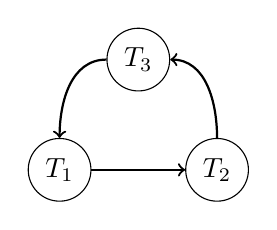
\begin{tikzpicture}
        [
            task/.style={circle, draw},
        ]
            \node[task] (T1) at (0.0, 0.0) {$T_1$};
            \node[task] (T2) at (2.0, 0.0) {$T_2$};
            \node[task] (T3) at (1.0, 1.4) {$T_3$};
            
            \draw[->, thick, draw] (T1.east) to [out=0,in=180] (T2.west);
            \draw[->, thick, draw] (T2.north) to [out=90,in=0] (T3.east);
            \draw[->, thick, draw] (T3.west) to [out=180,in=90] (T1.north);
        \end{tikzpicture}
        \caption{Precedence graph for schedule 1}
        \label{fig:trans-schedule-1}
    \end{figure}
    Since the graph forms a cycle, schedule 1 is not conflict serializable.

    \colbreak

    In schedule 2 we see that $T_1$ reads $X$ whilst $T_2$ wants to write to
    $X$, so $T_1$ must wait for $T_3$. Likewise, $T_3$ wants to write to $Z$
    whilst $T_2$ also wants to write to $Z$, so $T_3$ must wait for $T_2$.
    \begin{figure}[H]
        \centering
        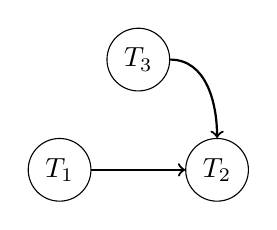
\begin{tikzpicture}
        [
            task/.style={circle, draw},
        ]
            \node[task] (T1) at (0.0, 0.0) {$T_1$};
            \node[task] (T2) at (2.0, 0.0) {$T_2$};
            \node[task] (T3) at (1.0, 1.4) {$T_3$};
            
            \draw[->, thick, draw] (T1.east) to [out=0,in=180] (T2.west);
            \draw[->, thick, draw] (T3.east) to [out=0,in=90] (T2.north);
        \end{tikzpicture}
        \caption{Precedence graph for schedule 2}
        \label{fig:trans-schedule-2}
    \end{figure}

\end{multicols}
